\subsection{Bestimmung der Mittleren Reichweite von $\alpha$-Strahlung} \label{sec:reichweite}
Für zwei Messreichen mit unterschiedlichem Abstand zwischen dem Detektor und dem Strahler wird zunächst die mittlere Reichweite von $\alpha$-Strahlung bestimmt. Die Abstände betragen
\begin{align*}
	x_{0,1} = \SI{2,1}{cm} \quad \text{und} \quad x_{0,2} = \SI{3,0}{\centi\meter} \, .
\end{align*}
Hierfür wird die Anzahl der Pulse über den effektiven Abstand vom Detektor zur Quelle
\begin{align}
	x = x_0 \frac{p}{p_0}
\end{align}
aufgetragen. Die Daten für Messung 1 sind in Tabelle~\ref{tab:messung1} zu finden und in Abbildung~\ref{fig:pulse1} dargestellt. Die Ergebnisse der zweiten Messung sind in Tabelle~\ref{tab:messung2} und Abbildung~\ref{fig:pulse2} zu sehen.  An die linearen Werte wird eine Ausgleichsgerade angelegt und mittels Python die Parameter für Steigung und y-Achsenabschnitt bestimmt
\begin{align}
	y = mx +b \quad .
\end{align}
Die Reichweite $R_m$ ist nun gerade die Strecke, bei der die Anzahl der maximal gezählten Pulse $P_\text{max}$  auf die Hälfte abgefallen ist
\begin{align}
	R_m = \frac{1}{m} \left(\frac{P_\text{max}}{2} -b \right) \quad .
\end{align}
Für die erste Messung folgen Werte
\begin{align}
	m_1 &= \input{build/m1.txt} \ , \\
	b_1 &= \input{build/b1.txt} \ , \\
	R_{m,1} &= \input{build/reichweite1.txt} \quad.
\end{align}
Und für die zweite Messung ergibt sich
\begin{align}
	m_2 &= \input{build/m2.txt} \ , \\
	b_2 &= \input{build/b1.txt} \ , \\
	R_{m,2} &= \input{build/reichweite2.txt} \quad.
\end{align}

\clearpage

 \begin{figure}[h!]
 	\centering
 	\captionof{table}{Messung 1 (Abstand \SI{2,1}{\centi\meter})}
 	\begin{tabular}{c|c|c}
 		Druck in \si{\milli\bar} & Pulse & effektive Länge in \si{cm} \\
 		\hline
 		\input{build/tabelle_messung1.txt}
 	\end{tabular}
 	\label{tab:messung1}
 \end{figure}

\begin{figure}[h!]
	\centering
	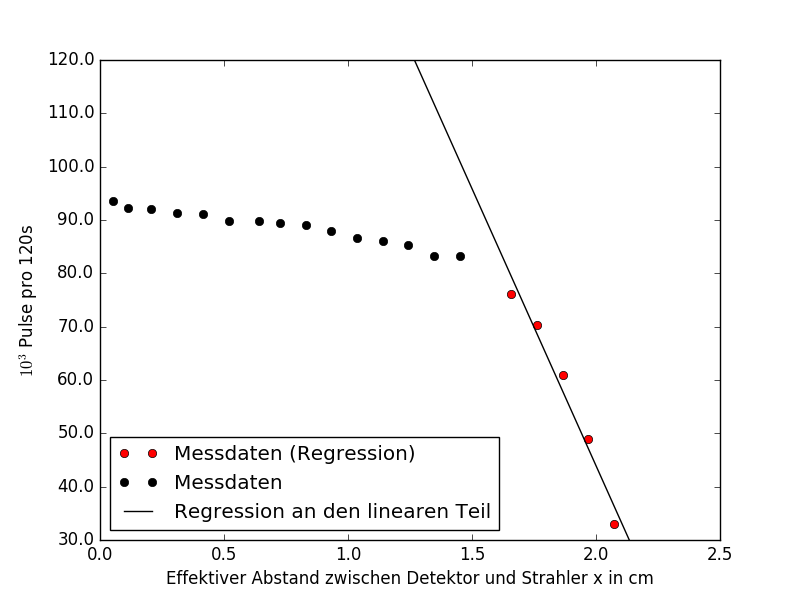
\includegraphics[width=0.75\textwidth]{build/pulse1.png}
	\caption{Messung 1 (Abstand \SI{2,1}{\centi\meter})}
	\label{fig:pulse1}
\end{figure}

\clearpage

 \begin{figure}[h!]
 	\centering
 	\captionof{table}{Messung 2 (Abstand \SI{3,0}{\centi\meter})}
 	\begin{tabular}{c|c|c}
 		Druck in \si{\milli\bar} & Pulse & effektive Länge in \si{cm} \\
 		\hline
 		\input{build/tabelle_messung2.txt}
 	\end{tabular}
 	\label{tab:messung2}
 \end{figure}
 
 \begin{figure}[h!]
 	\centering
 	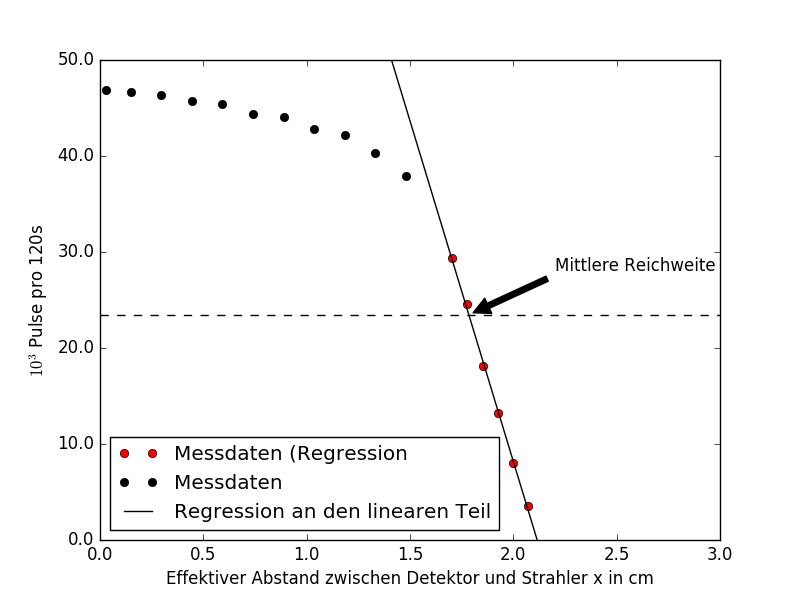
\includegraphics[width=0.75\textwidth]{build/pulse2.png}
 	\caption{Messung 2 (Abstand \SI{3,0}{\centi\meter})}
 	\label{fig:pulse2}
 \end{figure}
 
 \clearpage
 
 
 
 
 



\subsection{Bestimmung der Energie der $\alpha$-Strahlung}
Die Energie der $\alpha$-Strahlung kann auf zwei verschiedene Arten bestimmt werden. Die empirische Lösung
\begin{align}
	E_{\alpha, \text{emp}} = \left( \frac{R_m}{3.1} \right)^{2/3} \quad \text{($R_m$ in mm)}
\end{align}
mit Werten aus Kapitel~\ref{sec:reichweite}  liefert
\begin{align}
	E_{\alpha, \text{emp}, 1} &= \input{build/E1_emp.txt}\ , \\
	E_{\alpha, \text{emp}, 2} &= \input{build/E2_emp.txt} \quad .
\end{align}
Der zweite Lösungsweg geht über eine lineare Regression an die Energien bei verschiedenen effektiven Längen. Die Energien sind in \glqq Channel \grqq angegeben und müssen in \si{\mega\electronvolt} umgerechnet werden. Die Energie beim niedrigst möglichen Druck (im optimalen Fall \SI{0}{\milli\bar}) entspricht \SI{4}{\mega\electronvolt}. Die umgerechneten Energien sind in Tabelle~\ref{tab:energie1} und~\ref{tab:energie2} dargestellt. \\
Durch den linearen Anteil der Messdaten wird abermals ein Fit gelegt, um aus der Beziehung
\begin{align}
	E_{\alpha, \text{reg}} = - R_m \dv{E}{x} = - R_m m \quad \text{($R_m$ in cm)}
\end{align}
die Energie der $\alpha$-Teilchen zu erhalten. Für die Plots (Abbildung~\ref{fig:energie1} und~\ref{fig:energie2}) folgen die Werte
\begin{align}
	m_1 &= \input{build/m_e1.txt }\ , \\
	E_{\alpha, \text{reg}, 1}  &= \input{build/E1_reg.txt} \ , \\
	m_2 &= \input{build/m_e1.txt} \ , \\
	E_{\alpha, \text{reg}, 2} &=  \input{build/E2_reg.txt} \quad .
\end{align}

\clearpage


 \begin{figure}[h!]
 	\centering
 	\captionof{table}{Energien Messung 1 (Abstand \SI{2,1}{\centi\meter})}
 	\begin{tabular}{c|c|c}
 		Channel & Energie in \si{\mega\electronvolt} & effektive Länge in \si{cm} \\
 		\hline
 		\input{build/tabelle_energie1.txt}
 	\end{tabular}
 	\label{tab:energie1}
 \end{figure}
 
 
  \begin{figure}[h!]
  	\centering
  	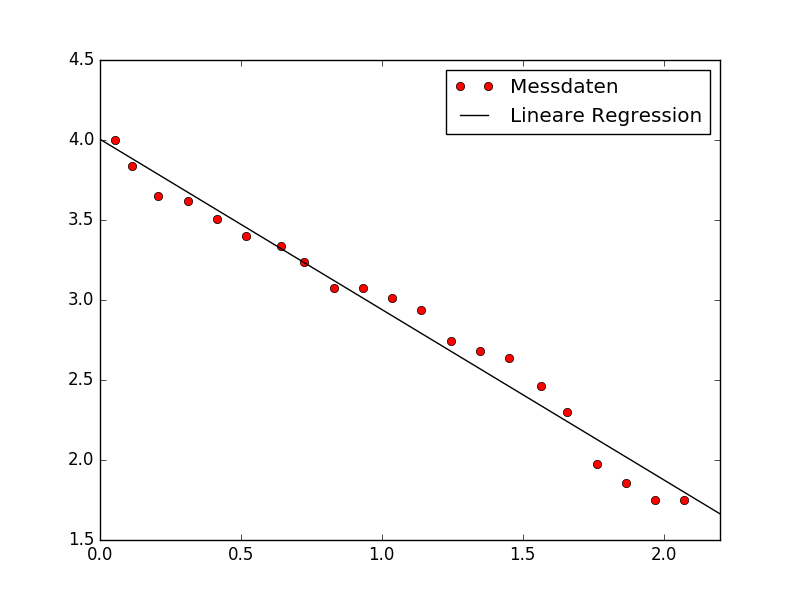
\includegraphics[width=0.75\textwidth]{build/energie1.png}
  	\caption{Energie der Messung 1 (Abstand \SI{2,1}{\centi\meter})}
  	\label{fig:energie1}
  \end{figure}
  
  \clearpage
  
  
    \begin{figure}[h!]
    	\centering
    	\captionof{table}{Energien Messung 2 (Abstand \SI{3,0}{\centi\meter})}
    	\begin{tabular}{c|c|c}
    		Channel & Energie in \si{\mega\electronvolt} & effektive Länge in \si{cm} \\
    		\hline
    		\input{build/tabelle_energie2.txt}
    	\end{tabular}
    	\label{tab:energie2}
    \end{figure}
    
   \begin{figure}[h!]
   	\centering
   	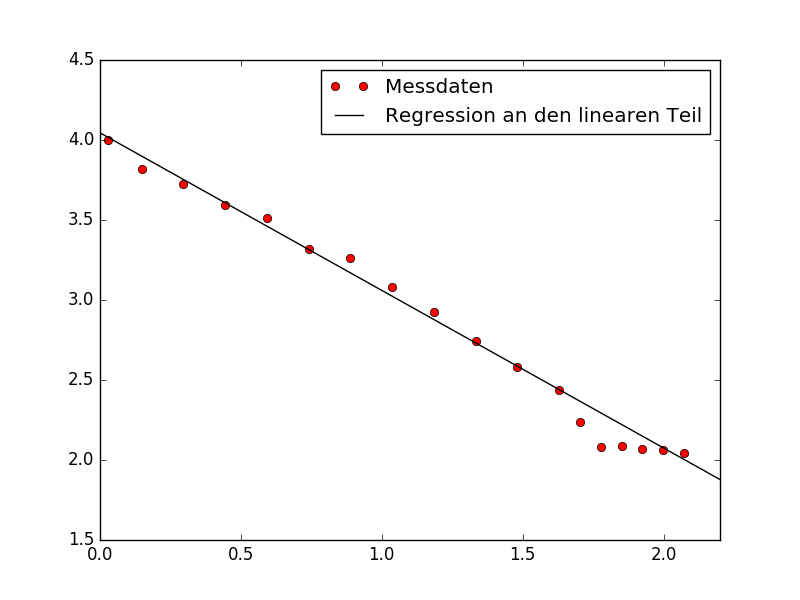
\includegraphics[width=0.75\textwidth]{build/energie2.png}
   	\caption{Energie der Messung 2 (Abstand \SI{3,0}{\centi\meter})}
   	\label{fig:energie2}
   \end{figure}
   
   
\clearpage


\subsection{Statistik des radioaktiven Zerfalls}
Aus 100 Messdaten wird eine Verteilung der Pulse erstellt, die innerhalb zehn Sekunden gemessen werden.
 



